\subsection{Where reaction stands}
\label{sec:reaction}
The alternative to forecasting is to react. On the full Mooncake traces, reactive tiering
reaches 75--99\% of Belady's hit rate on the toolagent trace and 40--94\% on open-ended conversation
using LRU, LFU or a fill-once cache alone; admitting the adaptive and learned policies below widens the
per-operating-point envelope only to 76--99\% and 42--94\% (\Cref{fig:reactive}). This section's metric is
a single cache's hit rate as a fraction of Belady's, with no move price, not the captured share of the
sections before it.

The interesting question is not the envelope --- that is an oracle over policies, not something anyone
deploys --- but whether any \emph{single} policy attains it, and whether the adaptive designs built for
exactly this situation beat plain rules. We therefore run the family: \textbf{ARC}~\cite{S7_megiddo2003arc},
which shifts a recency/frequency split on ghost hits; \textbf{LeCaR}~\cite{S8_vietri2018lecar} and
\textbf{CACHEUS}~\cite{S9_rodriguez2021cacheus}, which replace ARC's arithmetic update with regret-based
multiplicative weights over two experts; and the learned \textbf{LRB}, which is reported separately below because its
numbers carry an implementation band the others do not.

\begin{center}\small
\begin{tabular}{@{}lrrrrr@{}}
\toprule
trace & tier & best pure & ARC & LeCaR & CACHEUS \\
\midrule
conversation & 2\%  & 39.8 & 29.4 & \textbf{42.3} & 35.9 \\
             & 5\%  & 53.3 & \textbf{57.9} & 56.8 & 53.5 \\
             & 10\% & 76.0 & \textbf{77.5} & 77.2 & 75.3 \\
             & 20\% & \textbf{94.1} & 87.4 & 93.9 & 88.8 \\
\midrule
toolagent    & 2\%  & 74.9 & 70.7 & \textbf{75.8} & 73.9 \\
             & 5\%  & 81.3 & \textbf{83.6} & 83.0 & 82.9 \\
             & 10\% & 91.9 & 92.3 & \textbf{92.9} & 91.8 \\
             & 20\% & 99.3 & 96.3 & \textbf{99.3} & 97.6 \\
\bottomrule
\end{tabular}
\end{center}
\noindent{\footnotesize Percent of Belady's hit rate. ``Best pure'' is the best of LRU, LFU and a
fill-once cache (which admits blocks until it is full and never evicts) at that operating point, itself a choice
among policies, so the comparison is conservative for the adaptive designs.}

\medskip
\noindent Across eight operating points and four designs, \textbf{the best adaptive or learned policy
beats the best pure rule by at most 4.6 points of Belady}, and at the loosest tier by at most 0.1. Which
design wins also moves: LeCaR at the tightest tier on both traces and ARC at 5\%; above that, ARC and
then plain LRU on conversation, LeCaR on toolagent. That is the substantive finding --- not that these policies fail, but that on KV-block workloads
the whole adaptive-replacement family collapses into a band a few points wide, well short of the oracle
at the small tiers where the decision actually matters.

The diagnostics suggest why. Every policy in this family adapts
on a \emph{ghost hit} (a miss on a block it recently evicted), whether it updates a split (ARC) or
an expert weight (LeCaR, CACHEUS). But 76--78\% of blocks in these traces are never reused at all, so
most evictions are correct and produce no signal. Measured, ARC receives an adaptation signal on
\textbf{3.5--7.3\% of misses}; the regret-based policies read the same channel, which is why they land
in the same band rather than above it. What signal it does get is not merely sparse but, at
the smallest tier, directionally wrong: at a 2\% tier ARC drives $p$ to 90\% recency on both traces, while
the rule that actually wins there is frequency. A workload whose blocks are mostly singletons starves the
very mechanism adaptive replacement runs on.

The designs built for one-hit wonders do no better. S3-FIFO~\cite{yang2023s3fifo},
SIEVE~\cite{zhang2024sieve} and W-TinyLFU~\cite{einziger2017tinylfu}, reimplemented from their papers
(W-TinyLFU with exact, periodically halved counts in place of its sketch), stay below the best pure rule at
all eight operating points, by 0.1 to 8.9 points of Belady; the closest is W-TinyLFU at the tightest tier.
Quick demotion does what it was designed for: at the tightest tier S3-FIFO and W-TinyLFU beat LRU and ARC on
both traces. What they do not beat is the best plain rule chosen per operating point, and we did not
isolate why.

\paragraph{And the learned cache policy loses to both --- but only as a range} The natural learned
baseline is LRB~\cite{S6_song2020lrb}, which learns a relaxed-Belady objective from
a far richer feature set than our four trace-local statistics and won on production CDN traces. We
reimplement it: GBDT regression on log time-to-next-request over inter-access deltas and exponentially
decayed counters, sampled eviction, online retraining from a sliding memory window, right-censored
labels.

Our first version of it measured something else entirely. The training buffer was capped by truncating to
its tail; labelled rows arrive one at a time as blocks are re-accessed while censored rows arrive in one
contiguous burst per checkpoint, so from the third retrain onward every training label was identical, the
regressor returned a constant, and eviction degenerated to a uniform draw over the sampled candidates.
We report the repaired numbers and, because two defensible repairs disagree, we report them as a band:

\begin{center}\small
\begin{tabular}{@{}lrrrr@{}}
\toprule
trace & tier & LRB (repaired) & ARC & below ARC? \\
\midrule
conversation & 2\%  & 27.6--29.2 & 29.4 & yes \\
             & 5\%  & 30.9--32.2 & 57.9 & yes \\
             & 10\% & 45.0--45.9 & 77.5 & yes \\
             & 20\% & 75.8--76.5 & 87.4 & yes \\
\midrule
toolagent    & 2\%  & 68.8--69.0 & 70.7 & yes \\
             & 5\%  & 71.1--71.4 & 83.6 & yes \\
             & 10\% & 80.9--83.0 & 92.3 & yes \\
             & 20\% & 94.6--94.9 & 96.3 & yes \\
\bottomrule
\end{tabular}
\end{center}
\noindent{\footnotesize Percent of Belady, seed 0. The band spans two repairs of the truncation bug: subsampling
all accumulated rows, and dropping rows older than the memory window first. We adopt the second, which is
what a ``sliding memory window'' means.}

\medskip
\noindent \textbf{What the band supports.} The two repairs agree to within 2.1 points at every operating
point, and with seed 0 LRB is below ARC at all eight operating points under both. LRB samples its
eviction candidates and training rows at random, so we reran both repairs with ten seeds at the 2\% tier,
where the margins are smallest. The criterion we registered kept the ordering only if no seed reached ARC;
in three of the four trace--repair pairs one or two of ten seeds reach or pass it there, by at most 0.3
points of Belady, and the seeds spread LRB over up to 6.4 points on conversation. At that tier LRB and ARC are indistinguishable. The
claim we keep is narrower: \textbf{LRB does not beat ARC}, and it is below ARC by 9 points or more at five
of the other six operating points, more than the seed spread; at toolagent's 20\% tier the margin is 1.4
points, inside it. Both repairs and the retracted behaviour are selectable in the
artifact, so the band is regenerated rather than reported. We do not claim the band bounds every
reasonable reimplementation: a third repair produced in an AI-agent review we ran (see the Acknowledgments)
reported a figure at the 10\% conversation tier above our band but still below ARC; since
its code is not ours to ship, we neither reproduce nor rely on it.

The mechanism appears to be the one that limits ARC, seen from the other side. LRB learns from labels the
trace supplies when a sampled block is requested again; a block that never returns yields a
\emph{right-censored} row, which says only ``not within the window'' and nothing about when. At the
default window \textbf{83--88\% of LRB's training rows are censored}, and 88--91\% at a shorter one. A
population dominated by singletons starves the ghost-hit channel that adaptive replacement runs on and
the regression target that learned replacement runs on, for the same underlying reason.

Three caveats bound this. It is our reimplementation of the published mechanism, not the authors'
artifact. KV blocks are uniform-size, so byte miss ratio collapses to object miss ratio and LRB loses one
of its structural advantages over LRU. And our first hyperparameter sweep ran on the \emph{broken}
implementation, so it tested the robustness of random eviction. Rerun on the repaired one at a 10\%
tier (six settings of window, sample size and trees per trace), LRB spans 41.9--61.8\% of Belady on
conversation and 77.6--86.4\% on toolagent, below ARC's 77.5\% and 92.3\% at every setting; the band
is too wide to quote one LRB number, but not wide enough to reach ARC.


The eviction signal also inverts by source. On the agentic kv-cache-tester traces LRU reaches 0.83--0.96 of Belady at a 5\%
tier while LFU stays near 0.29--0.31; on Mooncake the ordering reverses below the working-set knee. An
eviction policy tuned on one source is a poor default for the other --- and, as both the ARC and the LRB
result show, reaching for a more sophisticated policy does not by itself resolve the choice.

\begin{figure}[t]
  \centering
  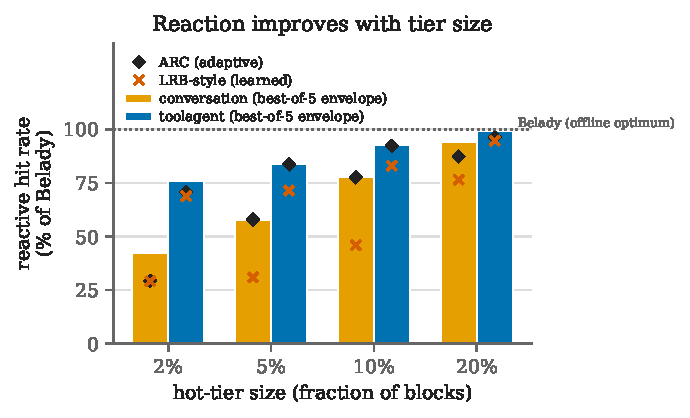
\includegraphics[width=\columnwidth]{fig_reactive.pdf}
  \caption{Reactive tiering as a fraction of Belady's hit rate, full Mooncake traces. Bars are a
  per-operating-point best-of-seven envelope, an oracle over policies rather than a policy. Diamonds are
  ARC, which meets the envelope at 5\% on both traces and at 10\% on conversation but falls short
  elsewhere; crosses are the
  LRB-style learned policy (seed 0), which is below ARC everywhere; other seeds reach ARC at the 2\% tier.}
  \label{fig:reactive}
\end{figure}
